\documentclass{article}


\usepackage{arxiv}

\usepackage[utf8]{inputenc} % allow utf-8 input
\usepackage[T1]{fontenc}    % use 8-bit T1 fonts
\usepackage{hyperref}       % hyperlinks
\usepackage{url}            % simple URL typesetting
\usepackage{booktabs}       % professional-quality tables
\usepackage{amsfonts}       % blackboard math symbols
\usepackage{nicefrac}       % compact symbols for 1/2, etc.
\usepackage{microtype}      % microtypography
\usepackage{lipsum}
\usepackage{fancyhdr}       % header
\usepackage{graphicx}       % graphics
\usepackage[table, x11names, svgnames]{xcolor}
\usepackage{subfig}
\usepackage[section]{placeins}
\usepackage{setspace}

\setstretch{1.2} % line spacing

\graphicspath{{assets/}}

%% Header
\pagestyle{fancy}
\thispagestyle{empty}
\rhead{ \textit{ }} 
\fancyhead[LO]{}

% \fancyhead[RE]{Firstauthor and Secondauthor} % Firstauthor et al. if more than 2 - must use \documentclass[twoside]{article}

%% Title
\title{Clinical advancement forecasting
%% Cite as
\thanks{\textit{\underline{Citation}}: 
\textbf{TBD}} 
}

%% Authors
\author{
  Authors TBD \\
  Related Sciences \\
%   %% examples of more authors
%    \And
%   Author3 \\
%   Affiliation \\
%   Univ \\
%   City\\
%   \texttt{email@email} \\
}

%% Body
\setlength{\parindent}{20pt}

\begin{document}
\maketitle

\begin{abstract}
This study examines the extent to which the outcomes of clinical trials can be predicted based on longitudinal properties of drug targets and diseases alone. We find that this is possible by comparing the historical performance of model-based target-disease pair prioritization methods to common baselines. Our primary objective is to demonstrate that statistical learning can effectively optimize such methods with no loss of interpretability. For example, non-negative linear models can produce simple weighting schemes across various types of human, animal and cell model evidence (for targets, diseases and pairings of the two) to identify target-disease pairs that advance beyond phase 2 trials with an average relative risk that is 2x higher than Open Targets composite scores. Other key characteristics of this study include: 1) a comprehensive longitudinal treatment of evidence as well as how it relates to leakage and reverse causality in biomedical research, 2) trial and/or drug details are not used in order to enable ranking for undeveloped targets/diseases, 3) analysis of the space of currently undeveloped, tractable targets with the highest likelihood of clinical success, 3) no data is used outside of Open Targets to ease reproduction and/or deployment, and 4) our method requires no expert knowledge and can easily support the inclusion of more lines of evidence over time, making it easy to operationalize.
% Note: OT multiplier (2x) taken from Sensitivity / Relative risk ratio distribution across configurations / mean@10
\end{abstract}

\section{Introduction}

It has been well established that drugs with human genetic evidence linking their respective targets to indications in clinical trials are more likely to succeed \cite{Nelson2015-eg,King2019-rc,Minikel2023.06.23.23291765,Razuvayevskaya2023.02.07.23285407,PMID:30652614,PMID:24833294,PMID:35804044,PMID:36963162}. This information has been used to devise many target and target-disease ranking algorithms based primarily on a synthesis of multiple genetic signals alone \cite{PMID:38172303,Koscielny2017-rr,PMID:31253980}. It is also possible to expand the breadth of this genetic support to more targets/diseases based on knowledge graphs, protein interactions and/or disease ontologies \cite{PMID:33262371,Bao2022-bq,Sadler2023-xd,PMID:36087372,PMID:36823319}. To our knowledge, all such expansion methods identify a larger space of opportunities at the expense of expected success rates. This is not a focus of this work as we aim, instead, to establish a framework for identifying targets/diseases with the very highest possible likelihood of success first. This is accomplished by integrating human clinical, genetic/genomic, transcriptomic and proteomic data as well as cell/animal model evidence, pathway information and basic literature metrics from Open Targets \cite{Koscielny2017-rr} in a simple statistical modeling framework. It can be contrasted with far more integrative methods that rely on neural and/or graph models over extensive knowledge graphs \cite{Paliwal2020-hr,PMID:33741907,pittala2020relationweighted,PMID:32750869}, which are more complex and difficult to interpret. We believe a desirable middle ground between these approaches and those that aim to combine many orthogonal indicators of success through expert knowledge in heuristic systems \cite{PMID:38404138,Koscielny2017-rr} would: 1) permit inclusion of many types of evidence from many sources, 2) be highly interpretable, 3) support expert judgement where necessary, and 4) not require manual ranking/weighting schemes.

A substantial challenge inherent to building such a system is the need to account for the longitudinal nature of knowledge discovery in biomedicine. This is vital because any method that optimizes for likely future clinical success based on historical clinical success may easily be biased by the non-random nature with which evidence is absent otherwise. We use only "temporalized" evidence, i.e. evidence for which timing of its emergence can be determined, and outcomes when training and evaluating our methods before ultimately applying them to present-day evidence with no restrictions on timing. We discuss motivations, prior research and our own analysis on how important this problem is for each source in Section~\ref{sec:results_inflation}.

Addressing such problems is common, but not ubiquitous, in studies that attempt to predict clinical trial outcomes using temporalized predictors \cite{PMID:37483175, PMID:34430930, Lo2019Machine}. The need for this is often clear in that setting where the inclusion of predictors like historical success rates for targets/diseases, trial sponsor track records, eventual patient enrollment, etc. constitute clear information leaks otherwise. This is discussed more in \cite{PMID:37483175} which notes several studies that do not account for this problem, and presents "quasi-prospective" as well as true "prospective" results. The difference between the two is that the former reconstructs timelines for predictors and outcomes based on recorded event dates while the latter relies on frozen predictions that are never evaluated until years later. Nomenclature for these formulations is conflicting though, where this definition of a "quasi-prospective" design is deemed entirely prospective in some cases, e.g. \cite{PMID:37225853}. We will refer to our design in this study as quasi-prospective since this definition is the best fit.

The prior works discussed so far can largely be categorized as either 1) target and target-disease prioritization methods evaluated based on how well they correlate with clinical trial success and 2) clinical trial outcome prediction models. Both are measured against the same outcomes and an important distinction between them lies in how the former methods are {\bf not} directly optimized for those outcomes while the latter methods are. In this study, we attempt to bridge these methodologies by predicting clinical trial advancement for target-disease pairs based solely on information that would be present well in advance of any drug program or individual trial. We then calibrate these predictions to determine what thresholds are necessary to match the observed success rates from benchmarks for genetic support like OMIM \cite{PMID:15608251}, ClinVar \cite{PMID:24234437} and GWAS. Finally, we examine how many present-day target-disease pairs are undeveloped (i.e. have never been in clinical trials), have a tractable target and are likely to see success rates matching or exceeding those calibrated benchmarks.

\section{Results}
\label{sec:results}

In order to model clinical advancement for target-disease (TD) pairs, we first define "advancement" as progression beyond any particular trial phase across all drugs associated with any one TD pair as indicated by the presence of a later-stage trial. All results to follow consider only advancement beyond phase 2 due to limitations described in Section~\ref{sec:discussion}. This binary outcome is then predicted based on a list of features shown in Supplementary~Table~\ref{tab:features}. Information for each of these features is only used when it was published before the year \textbf{prior} to the first phase 2 trial observed, with an exception for genetic evidence discussed in Section~\ref{sec:results_inflation}. A training dataset is then formed by including only TD pairs where this first phase 2 year is between 1990 and 2015. The evaluation dataset then consists of all TD pairs entering phase 2 between 2016 and 2022, with a 2 year offset from the present year (2024) to allow enough time for some trials to complete. While the average phase 2 trial duration may be as low as 2 years \cite{fdaStepClinical}, other estimates would suggest half of them take longer than 2.9 years \cite{PMID:29394327}. This means a substantial fraction of outcomes are censored, that this is an important parameter to test sensitivity to and that time itself is likely to be a crucial covariate in this formulation. The distribution of these outcomes, the number of associated targets/diseases and a variety of other statistics on this dataset are presented in Supplementary~Figure~\ref{fig:dataset_statistics}.

\subsection{Features}

The predictors used consist of 27 target-disease pair features, 5 target-specific features and 1 disease-specific feature. These are listed in Supplementary~Table~\ref{tab:features}. The target and disease specific features are chosen carefully such that they are either capable of being associated with years in which events supporting them occurred or result from large-scale, unbiased methods that do not favor well-studied or drugged targets/diseases. Examples of this include target-specific tissue expression specificity scores computed from Human Protein Atlas \cite{PMID:25613900} and LOEUF \cite{PMID:32461654} scores from gnomAD. Simply put, our dataset combines scores from Open Targets for target-disease evidence and a select subset of target prioritisation \cite{OT23.12release} fields with almost no modifications, other than to add target and disease specific indicators of maximum trial phases reached and two extra genetic association features.

\subsection{Models}

We train a variety of models including constrained and unconstrained linear and tree models. The constrained variants of these models force effects of all features to increase monotonically. This is possible with no feature transformations because all scores in Open Targets are constructed such that higher scores are presumed to be advantageous. We also apply these models to our evaluation dataset using several feature ablations in order to assess the value of groups of related features.

In order to compare these models to an Open Targets composite score, we use an equally weighted sum of all scores except for those assigned lower weights in \cite{OTweights}. Scores from these sources are multiplied by the corresponding weight before being summed.

\subsection{Performance}
\label{sec:results_performance}

Figure~\ref{fig:performance_across_ta} demonstrates how well our primary model in this study -- a constrained, linear L2-regularized model referred to from here on as "RDG" -- ranks TD pairs by comparison to a composite score from Open Targets ("OTS"). The relative risk (RR) metric used in this comparison as well as all others where not specified otherwise is defined as:

\begin{equation}
  \frac{P(advancement | rank >= N)}{P(advancement | rank < N)}.
\end{equation}

The third ranking method presented in Figure~\ref{fig:performance_across_ta}, "RDG-T", differs from the RDG model only in that it also uses time since the phase 2 transition as a predictive factor as well as all others. We observe that the use of this information almost universally improves standard performance metrics like ROC (receiver operating characteristic) and AP (average precision), however it adds little to no value in rankings beyond a level where substantial relative risk increases can be observed. In other words, it constitutes an effective but coarse mechanism for ranking TD pairs while lacking the high precision of other factors like genetic support. This is consistent with its nature as a necessary but not sufficient condition for success, and it is likely that much of the value it adds in the tail of lower rankings could be captured and enhanced if other early indicators for the many reasons trials fail \cite{Razuvayevskaya2023.02.07.23285407} were also included (see more on this in Section~\ref{sec:discussion}). As a more practical concern, we refrain from focusing on RDG-T, or the similar GBM-T model, because neither is readily applicable to undeveloped TD pairs for which the time since phase 2 transition is not available. They are, however, a useful performance ceiling towards which future work might build towards.

A subset of therapeutic areas was used for this analysis and this is reflected in both the mean estimates and distributions of Figure~\ref{fig:performance_across_ta}. A full list of these can be seen in Supplementary~Figure~\ref{fig:relative_risk_by_ta}, which also shows the RR estimates used in any summary statistics across therapeutic areas. These were selected based on criteria described in Section~\ref{sec:methods}. Lastly, Supplementary~Figure~\ref{fig:relative_risk_dist_across_ta} shows RR distributions by model with significances of their differences.

\begin{figure}[!htb]
  \centering
  \captionsetup{width=.9\linewidth}
  \subfloat[\centering]{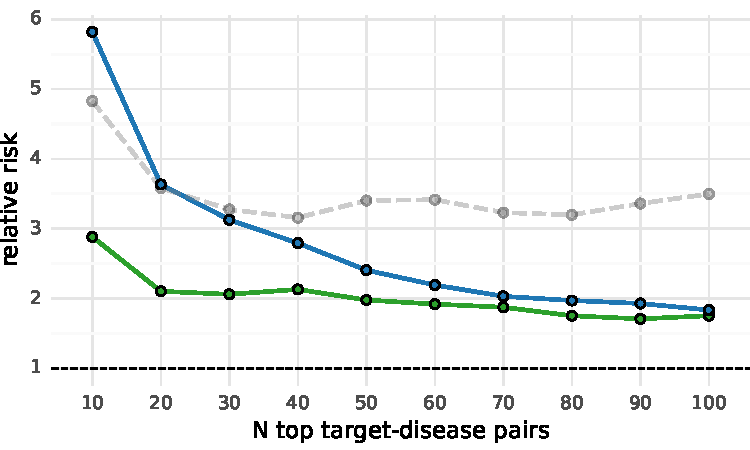
\includegraphics[width=.58\textwidth]{relative_risk_mean_across_ta.pdf}}
  \qquad
  \subfloat[\centering]{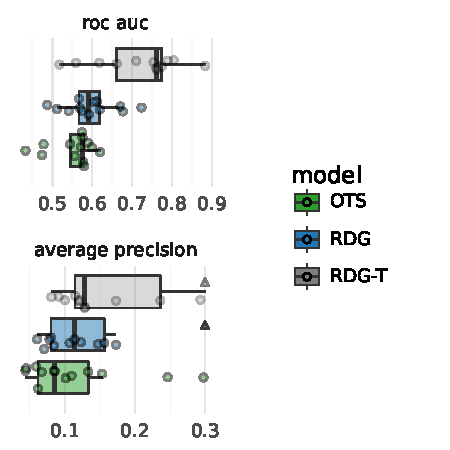
\includegraphics[width=.36\textwidth]{classifier_metrics_dist_across_ta.pdf}}
  \caption{
    \textbf{Statistical learning optimizes expected target-disease pair advancement rates using longitudinal evidence}.
    (a) Equally-weighted average relative risk estimates across 13 therapeutic areas, by number of top rankings and 3 methods: RDG (ours), RDG-T (ours) and Open Targets composite scores. 
    (b) Receiver operating characteristic (ROC) and average precision scores across the same 13 therapeutic areas with no limit on the number of rankings. 
    See Supplementary~Figure~\ref{fig:relative_risk_by_ta} for raw data underlying (a).
  }
  \label{fig:performance_across_ta}
\end{figure}

The relative risk estimates from the RDG model were also compared to univariate relative risk scores in Figure~\ref{fig:relative_risk_core_features}. This clearly implicates genetic features as being the most precise predictors, albeit with a relatively low frequency compared to others. Similar comparisons for target and disease specific features can be seen in Supplementary~Figure~\ref{fig:relative_risk_static_features}. These suggest that past clinical success for targets and diseases (independent of pairings) are likely to be highly predictive of advancement as well, while genetic constraint and expression specificity of targets also exhibit modest but significant effects.


\begin{figure}[!htb]
  \centering
  \captionsetup{width=.9\linewidth}
  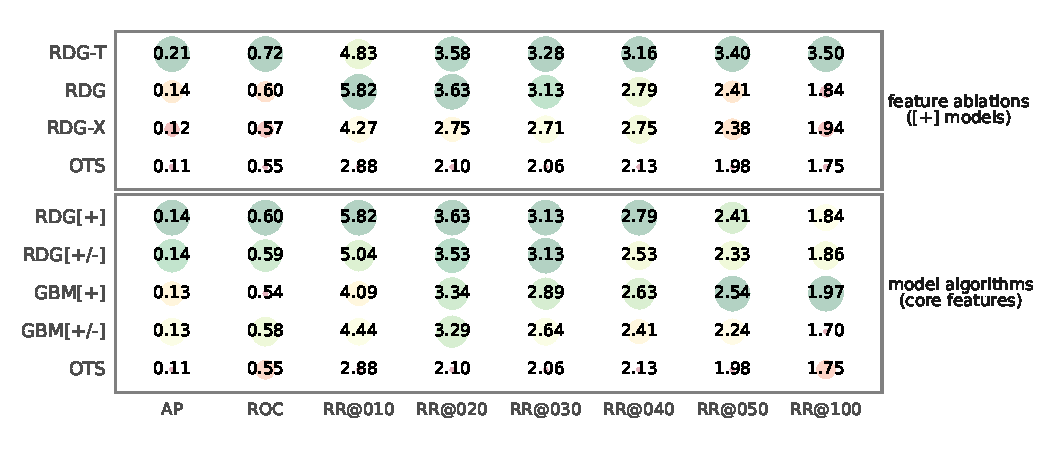
\includegraphics[width=1\textwidth]{performance_metric_mean_across_ta.pdf}
  \caption{
    \textbf{Performance of ...}.
  }
  \label{fig:performance_metric_mean_across_ta}
\end{figure}


In order to establish baseline levels of success and coverage across TD pairs, we refer to several of the univariate features in Figure~\ref{fig:relative_risk_core_features} throughout this study. Specifically, the \colorbox{Gainsboro}{omim} and \colorbox{Gainsboro}{ot\_genetics\_portal} features correspond to OMIM and GWAS baselines in the parlance of \cite{King2019-rc}, \cite{Nelson2015-eg} and \cite{Minikel2023.06.23.23291765}. We also use the \colorbox{Gainsboro}{eva} feature as a baseline for ClinVar support, which has discriminative capabilities somewhere between these two. The extent to which the RDG model meets or exceeds these benchmarks in both relative risk for advancement and TD pair coverage is illustrated in Figure~\ref{fig:relative_risk_by_limit}.

\begin{figure}[!htb]
  \centering
  \captionsetup{width=.9\linewidth}
  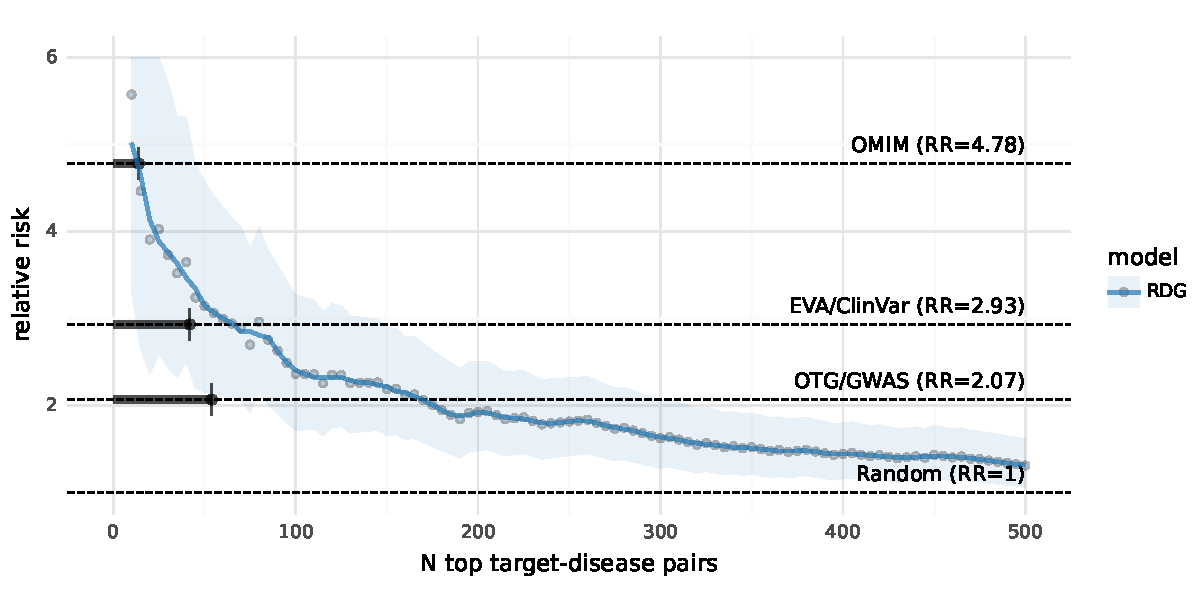
\includegraphics[width=1\textwidth]{relative_risk_by_limit.pdf}
  \caption{
    \textbf{RDG performance versus genetic support benchmarks across all therapeutic areas}. The RR estimates for each benchmark are based on the presence of the corresponding support across all TD pairs, and the number of pairs for which is present is represented by the horizontal bars extending horizontally from the y-axis. The bounds around the RDG RR estimates correspond to a 90\% confidence interval.
  }
  \label{fig:relative_risk_by_limit}
\end{figure}

One objective of this study is to determine if any model, e.g. RDG, could sort TD pairs with genetic support such that at least some portion of that sorted list had a likelihood of advancement that consistently exceeds what is expected from any one source of genetic support alone. As a hypothetical example, we wanted to determine if the top 50 TD pairs out of 200 with GWAS support were more likely to advance than all 200 overall. We find that this goal is met and exceeded by the RDG model, which actually identifies more TD pairs than those that have either EVA or GWAS support alone at an expected rate of advancement exceeding that of the single source (respectively). This does not appear to be the case with the OMIM baseline, however the lack of examples in our evaluation dataset with OMIM support makes any determination difficult. See Section~\ref{sec:results_opportunities} for more on how these benchmarks are employed to contextualize opportunities among undeveloped TD pairs.

\subsection{Sensitivity}

In order to validate the stability of our findings in Section~\ref{sec:results_performance}, we repeat this analysis across 18 different configurations listed in Supplementary~Table~\ref{tab:sensitivity_configurations}. This includes 3 separate versions of Open Targets, 3 choices for the year defining the split between training and evaluation data and 2 choices for the length of the minimum advancement window (in years).

We find that the mean RR values from the RDG model consistently exceed the OTS model in all configurations among the very highest rankings (N=10) and also exceed the OTS model in all configurations except for 1 for N between 20 and 60. This data is shown in Supplementary~Figure~\ref{fig:sensitivity_relative_risk}. The significance of these differences drops notably after N=40, which can be seen in the distribution of p-values from a Wilcoxon signed-rank test shown in Supplementary~Figure~\ref{fig:sensitivity_p_values}.

\subsection{Predictions}

Top predictions from the RDG model over the evaluation dataset are shown in Supplementary~Figure~\ref{fig:top_evaluation_predictions}. This figure demonstrates that there are a significant number of TD pairs with genetic support from many sources and that the combined effects of non-genetic features also substantially influence these rankings. 

\subsection{Effects}

The coefficients learned by the RDG model, and the average effects they have across the evaluation dataset, are shown in Figure~\ref{fig:effect_sizes}. This model most highly prioritizes genetic signals that have the greatest coverage, i.e. associations from GWAS studies through the \colorbox{Gainsboro}{ot\_genetics\_portal} feature and associations from any curated clinical genetics source, i.e. EVA, Orphanet, UniProt, Genomics England, ClinGen and gene2phenotype, via the \colorbox{Gainsboro}{curated} \vspace*{0mm} feature.  Notably, literature and target/disease specific clinical features also have substantial effects, followed by indicators of animal evidence and target genetic constraint / expression specificity. Any features not shown were deflated to have no effect, which is possible in this model due to the non-negativity constraint. One such feature worth emphasizing is transcriptomic evidence from Expression Atlas. We found this somewhat surprising, but it is supported by arguments against transcript over/under expression as an indicator of genes that influence disease rather than the other way around \cite{PMID:34561431}.

\begin{figure}[!htb]
	\centering
  \captionsetup{width=.9\linewidth}
	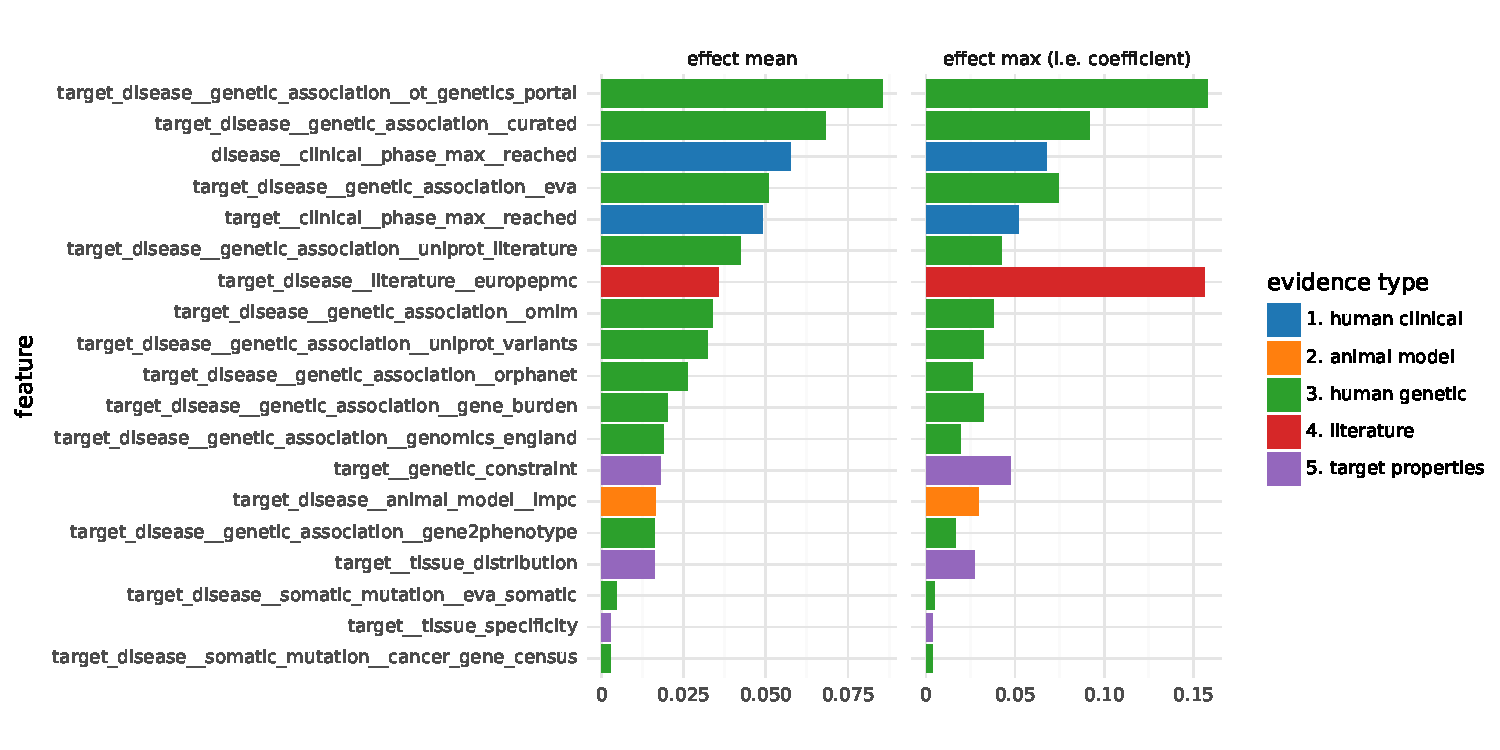
\includegraphics[width=1\textwidth]{effect_sizes.pdf}
  \caption{
    \textbf{RDG model feature effects}. The \textbf{effect max} values are equivalent to RDG model coefficients for the corresponding feature while the \textbf{effect mean} values indicate average values of the product between the coefficient and a particular feature value, when that feature is present.
  }
	\label{fig:effect_sizes}
\end{figure}

It is worth noting that the discordance between the coefficients and the average feature effects of Figure~\ref{fig:effect_sizes} arises from both the frequency with which features exist and the distribution of their underlying scores. Scores for many clinical genetics features (e.g. OMIM, Genomics England, UniProt) are very frequently absent or close to 1. By comparison, scores for literature associations are typically far lower, even when limited only to cases where they exist, with a median value of 0.12 (mean=.23) in the evaluation data.

\subsection{Opportunities}
\label{sec:results_opportunities}

A common method for identifying druggable opportunities within a specific disease context involves first ranking TD pairs according to some prioritization methodology followed by filtering or reprioritizing those ranks based on knowledge of target tractability \cite{PMID:28356508,PMID:35401535,PMID:31253980}. We use a similar approach to identify tractable targets associated with TD pairs that have yet to enter clinical trials. To aid in interpreting this approach, we also draw on the results of Figure~\ref{fig:relative_risk_by_limit}. The data in this figure suggests thresholds for the RDG model that align to expected rates of advancement compared to several genetic support benchmarks. These thresholds are used to bucket undeveloped TD pairs before further bucketing them based on levels of tractability. The tractability buckets in Supplementary~Table~\ref{tab:tractability_buckets} provide \colorbox{Gainsboro}{HIGH}, \colorbox{Gainsboro}{MED}, and \colorbox{Gainsboro}{LOW} confidence ratings for each type of tractability evidence based on the priorities suggested in \cite{OTTractability}.

\begin{figure}[!htb]
  \centering
  \captionsetup{width=.9\linewidth}
  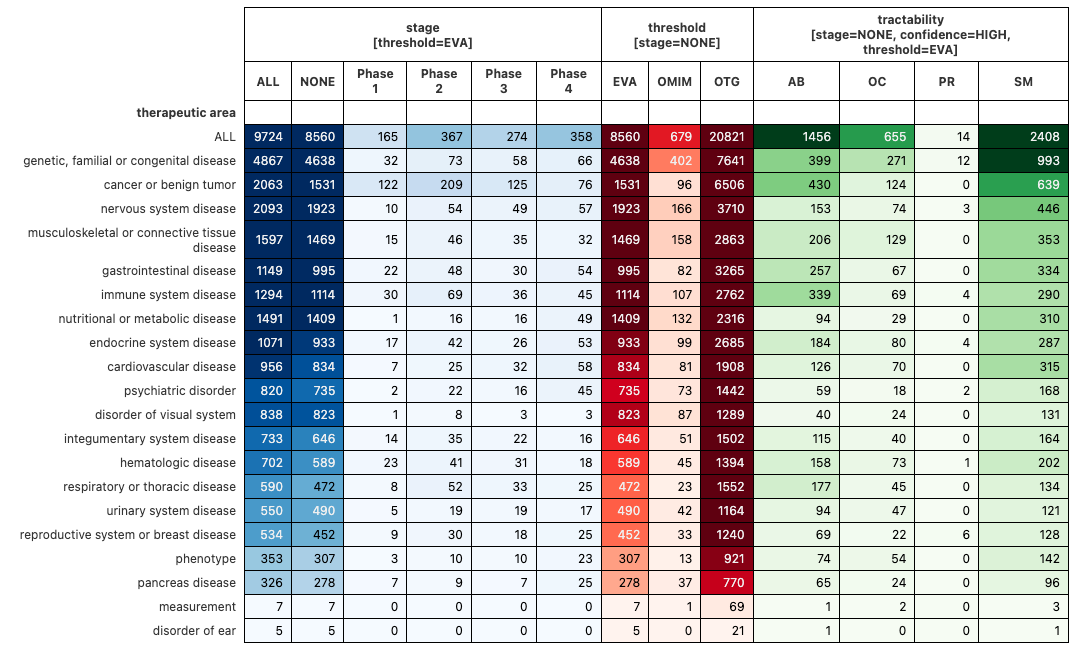
\includegraphics[width=1\textwidth]{opportunity_summary.png}
  \caption{
    \textbf{Present-day target-disease pair counts by tractability, likelihood of advancement and therapeutic area}. The \textbf{stage} panel contains counts by maximum trial phase reached, the \textbf{threshold} panel contains counts of pairs with a RDG model score exceeding that of the associated benchmark for only undeveloped pairs, and the \textbf{tractability} panel shows pair frequencies among undeveloped pairs exceeding the EVA threshold that also have a HIGH tractability rating as defined in Supplementary~Table~\ref{tab:tractability_buckets}. This corresponds to targets that have all been in clinical development already, except for the \textbf{OC} modality in which case it indicates that a target has been approved. 
  }
  \label{fig:opportunity_summary}
\end{figure}

Figure~\ref{fig:opportunity_summary} shows the distribution of TD pair counts for select buckets across therapeutic areas as well as across the current maximum phase reached for any one pair. We find that there are $\sim$2,400 small-molecule-enabled, $\sim$1,400 antibody-enabled, and 14 PROTAC-enabled TD pairs with a probability of advancement that is nearly 3x other TD pairs based on the EVA threshold RR=2.93 in Figure~\ref{fig:relative_risk_by_limit}. Top antibody-enabled pairs are shown in Supplementary~Figure~\ref{fig:top_opportunity_predictions} along with their corresponding genetic and clinical support.

\subsection{Algorithms}

The primary model for this analysis, RDG, is a constrained, L2-regularized linear regressor. Alternatives to this choice we explore include constrained and unconstrained gradient-boosted machine (GBM) models fit with the LightGBM \cite{LightGBM} algorithm as well as unconstrained L2-regularized linear regressors (i.e. RDG with no constraints). The performance of these alternatives, as quantified by relative risk estimates among top predictions, is illustrated in Figure~\ref{fig:relative_risk_model_features}. 

\begin{figure}[!htb]
  \centering
  \captionsetup{width=.9\linewidth}
  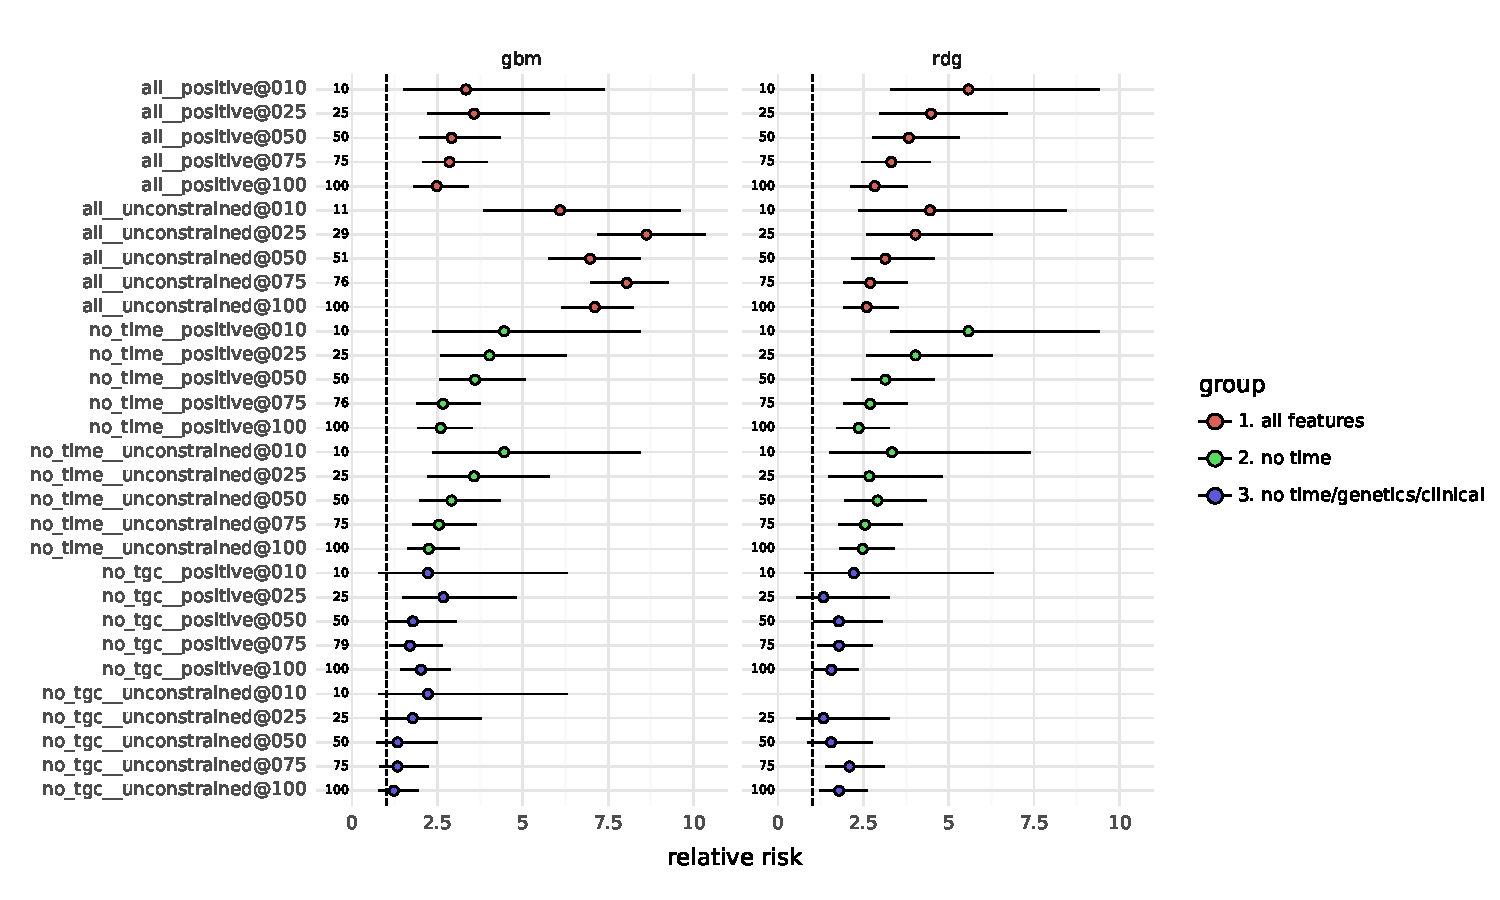
\includegraphics[width=1\textwidth]{relative_risk_model_features.pdf}
  \caption{
    \textbf{Performance by algorithm, constraint type and feature grouping}.  
  }
  \label{fig:relative_risk_model_features}
\end{figure}

We conclude from these results that 1) linear models outperform, or are at least not worse, than tree models when time is not used as a predictor and 2) non-negativity constraints in linear models result in greater performance. This is consistent with our expectation that all Open Targets scores should have monotonically increasing effects on the likelihood of success, since they were designed with this intent.

\subsection{Inflation}
\label{sec:results_inflation}

Like most studies of this kind, we assume a "closed-world" \cite{Paliwal2020-hr} over the space of target-disease pairs and any evidence between them. This means that we do not differentiate between evidence that an association for any one pair truly does \textbf{not} exist (or is too weak to be relevant under the omnigenic model \cite{PMID:28622505}), and the lack of any attempt to find that evidence in the first place. This also means that our estimate of the prognostic value for any one evidence source is subject to historical trends in biomedical research and the myriad ways that this research can be biased towards particular targets and diseases. We avoid attempting to comprehensively survey these biases in favor of offering an illustrative list of specific examples that are relevant in this study:

\begin{enumerate}
\item Mendelian randomization research is biased towards cardiovascular diseases as they have a disproportionate number of known, modifiable exposures \cite{PMID:36736292}
\item Putative protein interactions that do not result from genome-scale or otherwise unbiased assays result in an overrepresentation of successful drug targets in resources like STRING \cite{PMID:36370105}, thereby inflating the success of network expansion methods over these databases to identify such targets \cite{Sadler2023-xd}.
\item Transcript expression studies run in late-stage clinical trials for a single indication, e.g. \cite{PMID:27723281} linking SLE to IFN genes, are a degenerate indicator of advancement beyond earlier stage trials when the timing of this evidence is not accounted for.
\item Targets tested against more indications in clinical trials enrich for failures because the marginal cost of testing more indications decreases, but the evidence for these indications is often weaker \cite{PMID:33262371}.
\item Herding effects in pharma R\&D pipelines around particular drug targets are becoming increasingly clear over time \cite{PMID:37117303} and generate an excess of clinical evidence for those targets.
\end{enumerate}

We also note that the skew in basic drug target research towards those that already have rich annotations and well characterized molecular function \cite{PMID:29358745} as well as the disproportionate representation of particular target families in pharma R\&D pipelines \cite{PMID:27910877,PPR:PPR7029} and the fact that literature is well known to be biased away from negative results in general \cite{PMID:32893970} are all problematic. 

While it is not possible to address all of these issues, we emphasize that there is a clear pattern across the examples in the list above in that they require \textbf{past} clinical successes and/or failures to arise in the first place. This suggests that accounting for when evidence first emerged would limit the extent of these problems. We do so in this study based solely on publication dates associated with any one piece of information linking target-disease pairs. This also offers a novel opportunity to attempt to quantify what kind of evidence suffers most from these biases. Figure~\ref{fig:evidence_inflation} presents results for this based on a relative risk statistic defined as:

\begin{equation}
  \frac{P(A | B)}{P(A | \neg B)}
\end{equation}

where:

\begin{itemize}
\item \(A\) is the event that evidence for a TD pair arises after its first early-stage (phase 1 or 2) trial rather than before
\item \(B\) is the event that a TD pair advances into late-stage trials (phase 3 or 4)
\end{itemize}

We refer to this as "inflation risk" so as not to confuse it with the relative risk statistic used in all other contexts, and it can be more simply described as the fraction of TD pairs for which evidence arises \textbf{after} the beginning of an ultimately successful early-stage trial divided by that same fraction for TD pairs that do not advance to late-stage trials. The intuition for this statistic is that it will be higher if successful trials lead to the generation of evidence of a particular type, and it should be 1 in cases where the emergence of evidence is independent of clinical success. We also measure this potential lack of independence through the more commonly used Fisher's exact test, e.g. \cite{PMID:19725948}, and both are presented in Figure~\ref{fig:evidence_inflation}.

\begin{figure}[!htb]
  \centering
  \captionsetup{width=.9\linewidth}
  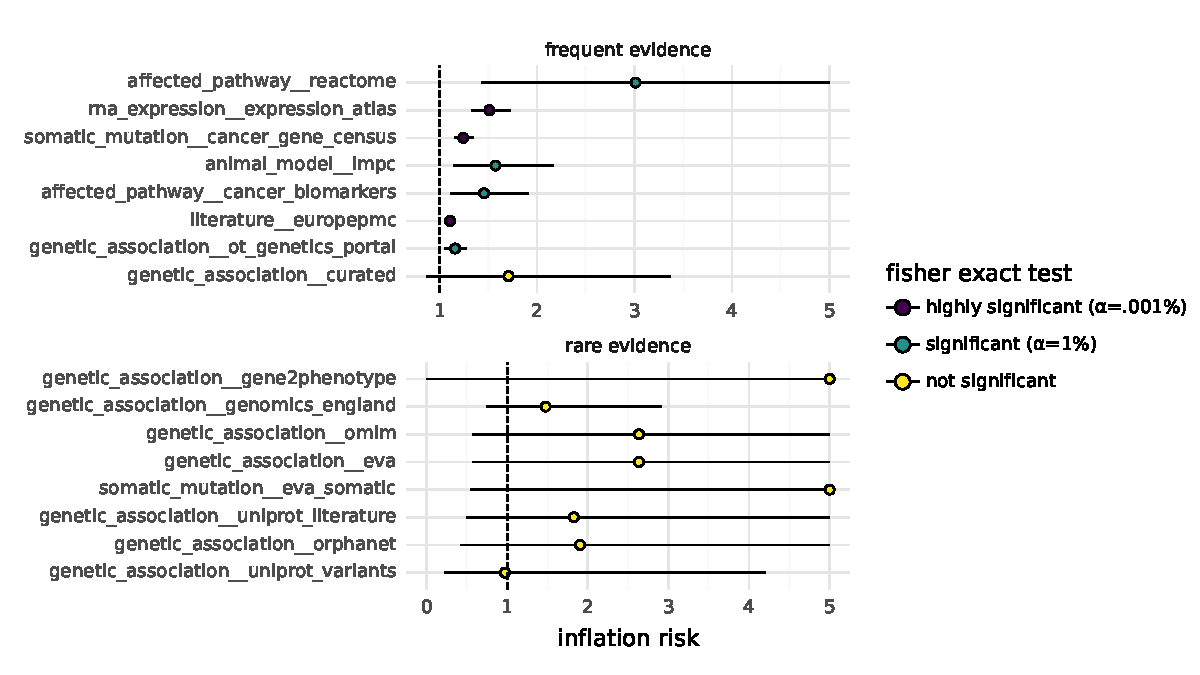
\includegraphics[width=1\textwidth]{evidence_inflation.pdf}
  \caption{
    \textbf{Clinical success drives evidence discovery}.  
  }
  \label{fig:evidence_inflation}
\end{figure}

We find that evidence from Reactome is the worst offender by this metric, implying that it often only arises for TD pairs after a certain level of clinical success has been attained. We also find that long-running aggregators/curators of published research often focused on individual diseases/phenotypes, like Expression Atlas, IMPC, CGS and Cancer Biomarkers exhibit this form of inflation as well.

Sources of genetic evidence appear to be much less inflated, or have too little data to reach significance. This is to be expected for GWAS evidence arising from genome-wide, phenome-wide biobank consortia, however much of historical GWAS evidence is not phenome-wide. More context on how much this is likely to matter comes from \cite{PMID:37612393} in which it was estimated that as few as 6\% of 500 FDA-approved targets for non-cancer drugs arose from programs highly motivated by pre-existing genetic support and that "the remaining 94\% were probably identified using conventional pharmacology, biochemistry or molecular biology approaches". We then speculate that if the initiation of new drug programs was not historically motivated highly by the existence of genetic support, then the incentives for pursing new genetic evidence based on clinical and commercial success are likely to be minimized. This, in conjunction with existing precedent \cite{Nelson2015-eg,King2019-rc,Minikel2023.06.23.23291765,Razuvayevskaya2023.02.07.23285407,PMID:30652614,PMID:35804044} and our inflation results, ultimately led us to the use of genetic evidence without temporalization. In other words, we do not treat genetic evidence as longitudinal features like all others associated with TD pairs. A breakdown of which features are treated in which manner is provided in Supplementary~Table~\ref{tab:features}.

\section{Conclusion}

We have demonstrated that simple machine learning methods applied to longitudinal biomedical evidence from many sources can be used to predict clinical outcomes for combinations of drug targets and diseases, without knowledge of molecular properties or trial design details. We have also shown that these methods are more precise in the extremes of their predictions than composite, heuristic scores like those from Open Targets. They also outperform such baselines by more comprehensive, traditional measures of classifier performance; however, we find this less compelling and easier to accomplish than improving performance among the upper tail of the opportunities implied by the very highest predictions. This framework would also support the addition of new lines of evidence over time well as it is designed to automatically determine the relevance of any new information without intervention.  Lastly, we find that the space of present-day, undeveloped targets within a disease context that both exceed baseline levels of tractability and have a high predicted likelihood of clinical advancement is substantial. It is likely to grow quickly as well since the breadth of much of the underlying evidence is expanding rapidly \cite{PMID:33214558,PMID:36634672,PMID:31491408}.

\section{Discussion}
\label{sec:discussion}

\begin{itemize}
  \item Cover limitations with OT concerning temporalization for both evidence and drug approvals, and why only transitions from phase 2 are relevant for this work
  \item Discuss the possibility to do prospective evaluation with OT snapshots
  \item Discuss how typical classifier metrics are inadequate for this problem
  \item Talk about how the inclusion of time greatly improves performance and suggests it may be possible to fill in this proxy with predictors for more specific early indicators of other reasons trials fail
  \item We are focusing on prioritizing among targets/indications with genetic support, rather than expanding this space to find opportunities with weaker support
  \item "There is evidence that a 9.6\% vs. 13.8\% success rate for drugs from phase 1 trials to approval may mean a \$480 million difference in the median research and development cost required to bring a new drug to the market (Wouters, McKee, and Luyten 2020)." \cite{PMID:34930919}
  \item From \cite{PMID:33262371}: "It is important to bear in mind therefore that what we are measuring when looking at historical trial outcomes is not an unbiased measure of any given gene's true disease associations, but rather a view on how useful a given evidence source or analytical method has been for choosing drug targets based on current and historical drug discovery practices. Dramatic changes in these practices in the future could render some of our conclusions obsolete, though the fundamental observation that genetic association itself is retained in molecular networks will remain valid."
  \item Add select tractability and DepMap features?
\end{itemize}

\section{Methods}
\label{sec:methods}

\begin{itemize}
  \item Discuss why all target prioritisation data fields are not used due to the potential leakage they may impose (e.g. target families, GO annotations, etc.)
  \item Describe how therapeutic areas were selected based on having at least 100 TD pairs with target-disease-specific evidence of any kind and with explicit omissions: ("biological\_process", "pregnancy or perinatal disease", "injury, poisoning or other complication", "pregnancy or perinatal disease", "medical procedure", "infectious disease", "animal disease")
  \item Training/evaluation results are limited by temporalization while the present-day predictions are not
  \item OMIM is defined as EVA associations with publications
  \item The "genetic\_association\_\_curated" field is a union of all genetic association sources other than "gene\_burden" and "ot\_genetics\_portal"
  \item Mention that the scores for a TD pairs in a year are the maximum score for that source, not the harmonic sum
  \item Mean imputation is used for target-specific features
  \item Mention specifics on RDG and GBM implementations, i.e. lightGBM and scikit-learn
  \item RDG is always trained on all features, but only applied to feature subsets where relevant
\end{itemize} 

\section{Supplementary Material}

\begin{table}
\centering
\caption{Features used in modeling and analysis}
\label{tab:features}
\begin{tabular}{llll}
\toprule
 & feature & entity & kind \\
\midrule
1 & disease\_\_clinical\_\_phase\_max\_\_reached & disease & temporal \\
2 & target\_\_clinical\_\_phase\_max\_\_reached & target & temporal \\
3 & target\_\_genetic\_constraint & target & static \\
4 & target\_\_mouse\_ko\_score & target & static \\
5 & target\_\_tissue\_distribution & target & static \\
6 & target\_\_tissue\_specificity & target & static \\
7 & target\_disease\_\_affected\_pathway\_\_cancer\_biomarkers & target\_disease & temporal \\
8 & target\_disease\_\_affected\_pathway\_\_crispr & target\_disease & temporal \\
9 & target\_disease\_\_affected\_pathway\_\_crispr\_screen & target\_disease & temporal \\
10 & target\_disease\_\_affected\_pathway\_\_progeny & target\_disease & temporal \\
11 & target\_disease\_\_affected\_pathway\_\_reactome & target\_disease & temporal \\
12 & target\_disease\_\_affected\_pathway\_\_slapenrich & target\_disease & temporal \\
13 & target\_disease\_\_affected\_pathway\_\_sysbio & target\_disease & temporal \\
14 & target\_disease\_\_animal\_model\_\_impc & target\_disease & temporal \\
15 & target\_disease\_\_genetic\_association\_\_clingen & target\_disease & static \\
16 & target\_disease\_\_genetic\_association\_\_curated & target\_disease & static \\
17 & target\_disease\_\_genetic\_association\_\_eva & target\_disease & static \\
18 & target\_disease\_\_genetic\_association\_\_gene2phenotype & target\_disease & static \\
19 & target\_disease\_\_genetic\_association\_\_gene\_burden & target\_disease & static \\
20 & target\_disease\_\_genetic\_association\_\_genomics\_england & target\_disease & static \\
21 & target\_disease\_\_genetic\_association\_\_omim & target\_disease & static \\
22 & target\_disease\_\_genetic\_association\_\_orphanet & target\_disease & static \\
23 & target\_disease\_\_genetic\_association\_\_ot\_genetics\_portal & target\_disease & static \\
24 & target\_disease\_\_genetic\_association\_\_uniprot\_literature & target\_disease & static \\
25 & target\_disease\_\_genetic\_association\_\_uniprot\_variants & target\_disease & static \\
26 & target\_disease\_\_known\_drug\_\_chembl & target\_disease & temporal \\
27 & target\_disease\_\_literature\_\_europepmc & target\_disease & temporal \\
28 & target\_disease\_\_outcome\_\_advanced & target\_disease & temporal \\
29 & target\_disease\_\_rna\_expression\_\_expression\_atlas & target\_disease & temporal \\
30 & target\_disease\_\_somatic\_mutation\_\_cancer\_gene\_census & target\_disease & temporal \\
31 & target\_disease\_\_somatic\_mutation\_\_eva\_somatic & target\_disease & temporal \\
32 & target\_disease\_\_somatic\_mutation\_\_intogen & target\_disease & temporal \\
33 & target\_disease\_\_time\_\_transition & target\_disease & temporal \\
\bottomrule
\end{tabular}
\end{table}


\begin{table}
\centering
\caption{Tractability bucket assignments}
\label{tab:tractability_buckets}
\begin{tabular}{llll}
\toprule
 & evidence & modality & confidence \\
\midrule
1 & Phase 1 Clinical & OC & LOW \\
2 & Advanced Clinical & OC & MED \\
3 & Approved Drug & OC & HIGH \\
4 & GO CC med conf & AB & LOW \\
5 & Human Protein Atlas loc & AB & LOW \\
6 & UniProt SigP or TMHMM & AB & LOW \\
7 & UniProt loc med conf & AB & LOW \\
8 & GO CC high conf & AB & MED \\
9 & UniProt loc high conf & AB & MED \\
10 & Advanced Clinical & AB & HIGH \\
11 & Approved Drug & AB & HIGH \\
12 & Phase 1 Clinical & AB & HIGH \\
13 & Database Ubiquitination & PR & LOW \\
14 & Half-life Data & PR & LOW \\
15 & Small Molecule Binder & PR & LOW \\
16 & Literature & PR & MED \\
17 & UniProt Ubiquitination & PR & MED \\
18 & Advanced Clinical & PR & HIGH \\
19 & Phase 1 Clinical & PR & HIGH \\
20 & Druggable Family & SM & LOW \\
21 & High-Quality Pocket & SM & LOW \\
22 & Med-Quality Pocket & SM & LOW \\
23 & High-Quality Ligand & SM & MED \\
24 & Structure with Ligand & SM & MED \\
25 & Advanced Clinical & SM & HIGH \\
26 & Approved Drug & SM & HIGH \\
27 & Phase 1 Clinical & SM & HIGH \\
\bottomrule
\end{tabular}
\end{table}


\begin{table}
\centering
\caption{Configurations for sensitivity analysis}
\label{tab:sensitivity_configurations}
\begin{tabular}{llrr}
\toprule
 & open\_targets\_version & max\_training\_year & min\_time\_to\_advancement\_years \\
\midrule
1 & 23.09 & 2017 & 4 \\
2 & 23.12 & 2017 & 2 \\
3 & 23.09 & 2015 & 2 \\
4 & 23.12 & 2015 & 2 \\
5 & 23.09 & 2017 & 2 \\
6 & 23.06 & 2015 & 4 \\
7 & 23.06 & 2017 & 2 \\
8 & 23.06 & 2013 & 2 \\
9 & 23.06 & 2015 & 2 \\
10 & 23.06 & 2017 & 4 \\
11 & 23.12 & 2013 & 4 \\
12 & 23.09 & 2015 & 4 \\
13 & 23.09 & 2013 & 2 \\
14 & 23.12 & 2013 & 2 \\
15 & 23.09 & 2013 & 4 \\
16 & 23.12 & 2017 & 4 \\
17 & 23.12 & 2015 & 4 \\
18 & 23.06 & 2013 & 4 \\
\bottomrule
\end{tabular}
\end{table}


\begin{figure}
  \centering
  \captionsetup{width=.9\linewidth}
  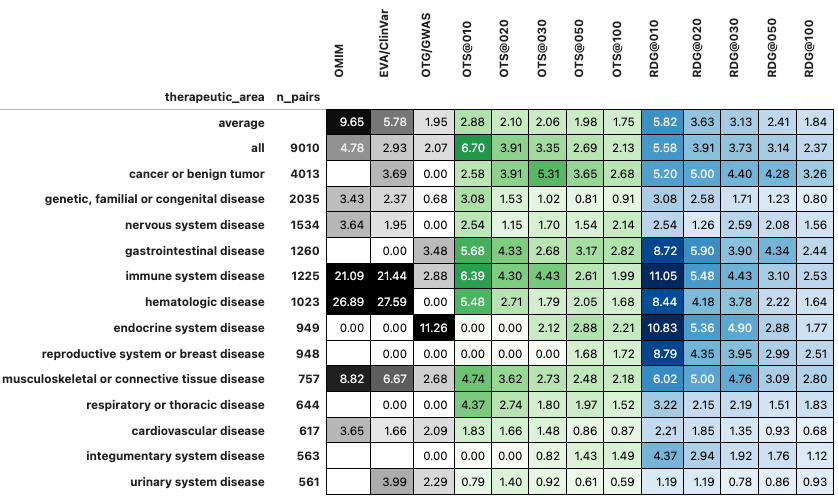
\includegraphics[width=1\textwidth]{relative_risk_by_ta.png}
  \caption{
    \textbf{Relative risk scores by method, benchmark and therapeutic area}.
    The \textbf{average} therapeutic area indicates mean values across all others except for \textbf{all}, which is an ungrouped estimate across all diseases regardless of therapeutic area.
  }
  \label{fig:relative_risk_by_ta}
\end{figure}


\begin{figure}
  \centering
  \captionsetup{width=.9\linewidth}
  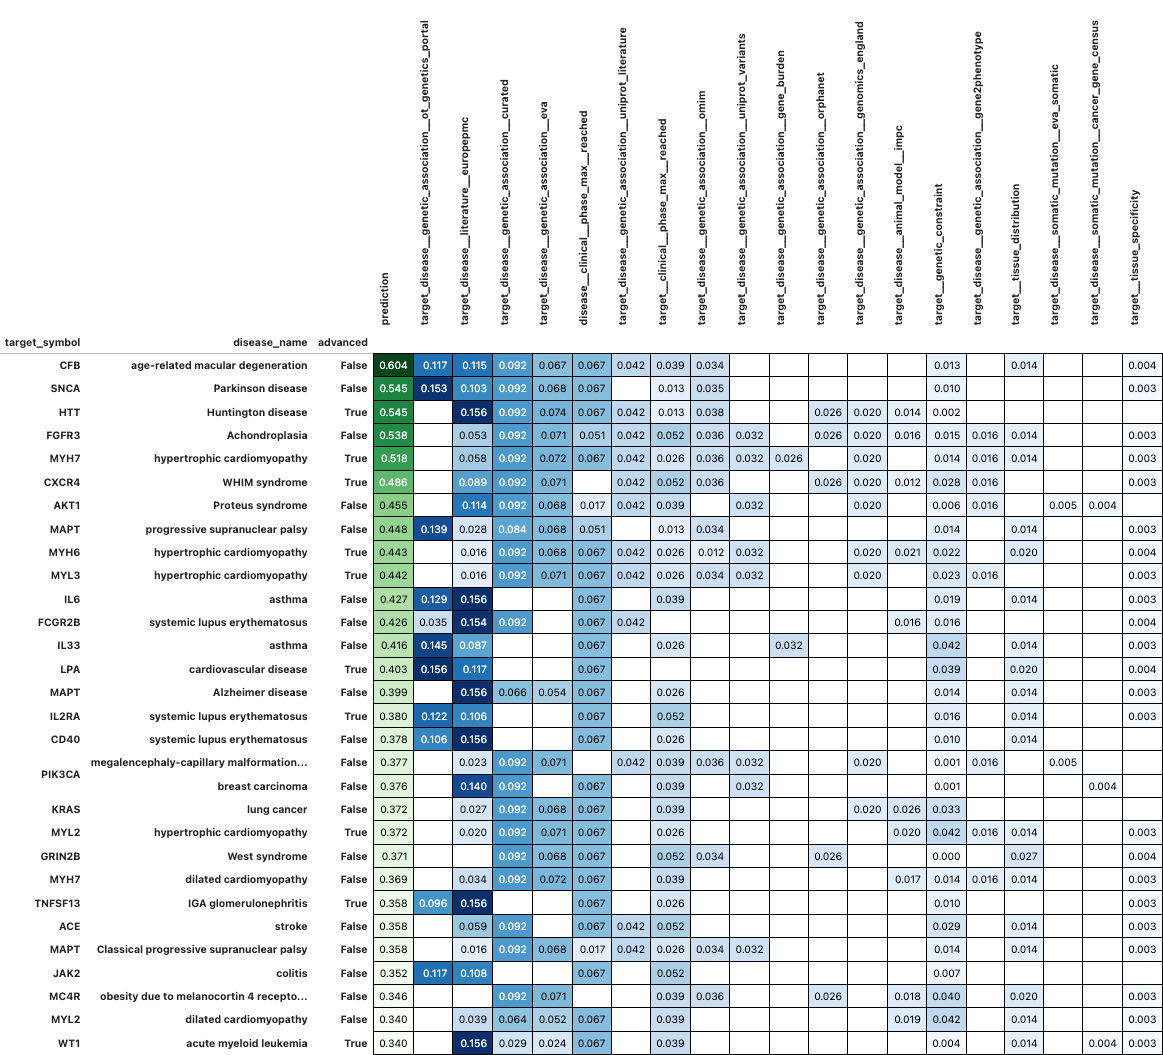
\includegraphics[width=1\textwidth]{top_evaluation_predictions.png}
  \caption{
    \textbf{Top RDG model evaluation dataset predictions}.
    Feature contributions are shown as the product of their underlying values and the RDG coefficients. The \textbf{advanced} field indicates whether the associated TD pair advanced beyond phase 2 as of 2024.
  }
  \label{fig:top_evaluation_predictions}
\end{figure}

\begin{figure}
  \centering
  \captionsetup{width=.9\linewidth}
  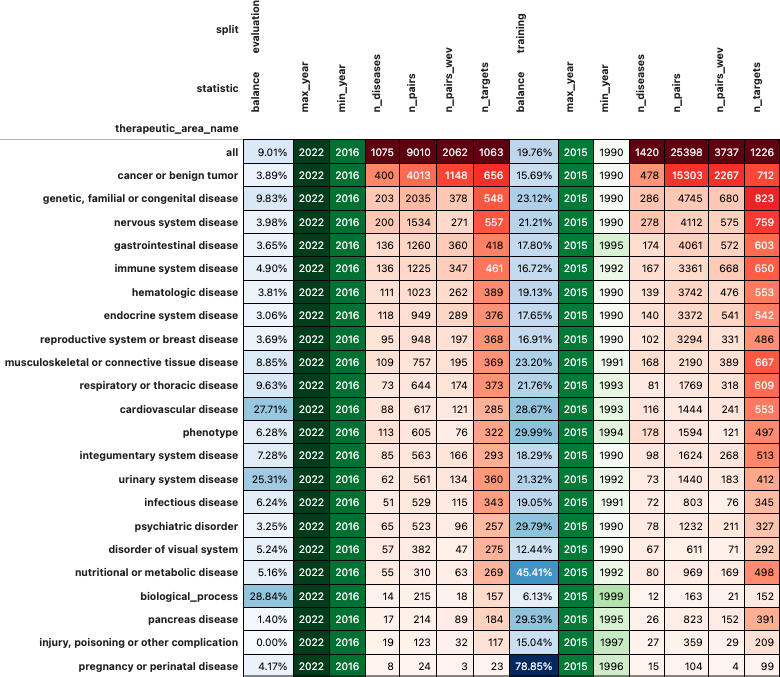
\includegraphics[width=1\textwidth]{dataset_statistics.png}
  \caption{
    \textbf{Training and evaluation dataset summary statistics}.
  }
  \label{fig:dataset_statistics}
\end{figure}
  
\begin{figure}
  \centering
  \captionsetup{width=.9\linewidth}
  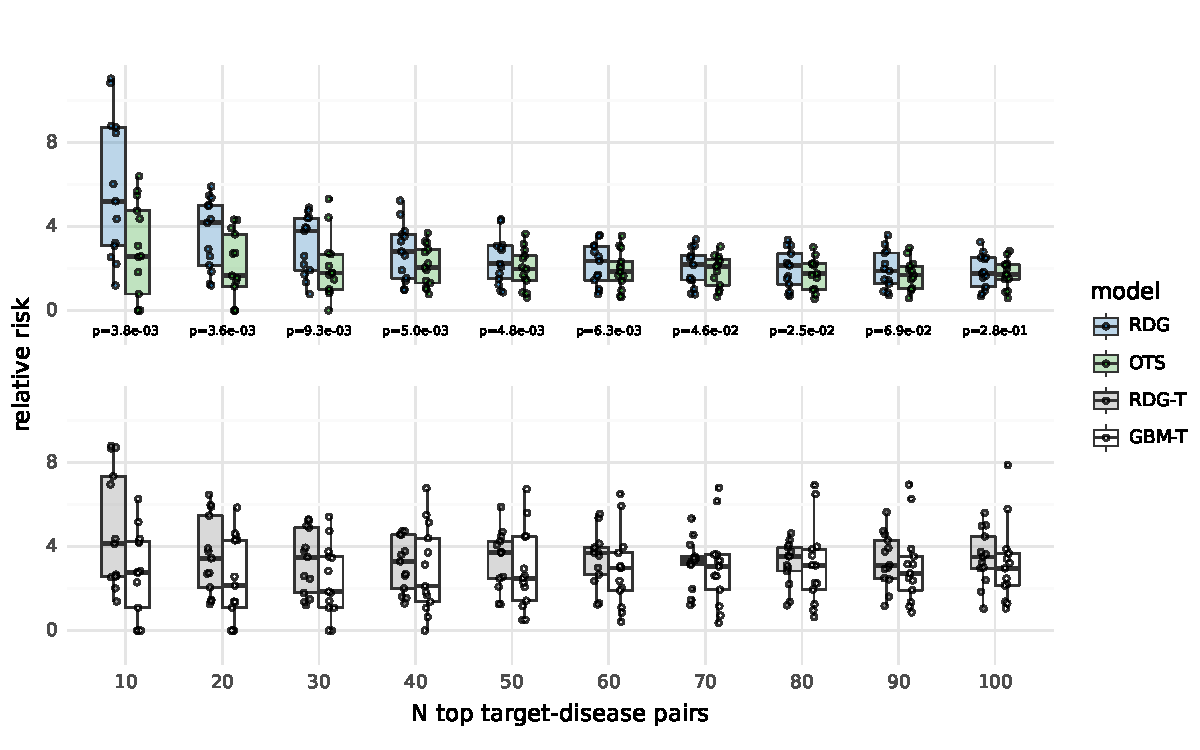
\includegraphics[width=1\textwidth]{relative_risk_dist_across_ta.pdf}
  \caption{
    \textbf{Relative risk distributions across select therapeutic areas}.
    P-values are computed from a one-sided Wilcoxon signed-rank test with the alternative that the RDG model RR averages across therapeutic areas exceed OTS averages.
  }
  \label{fig:relative_risk_dist_across_ta}
\end{figure}


\begin{figure}
  \centering
  \captionsetup{width=.9\linewidth}
  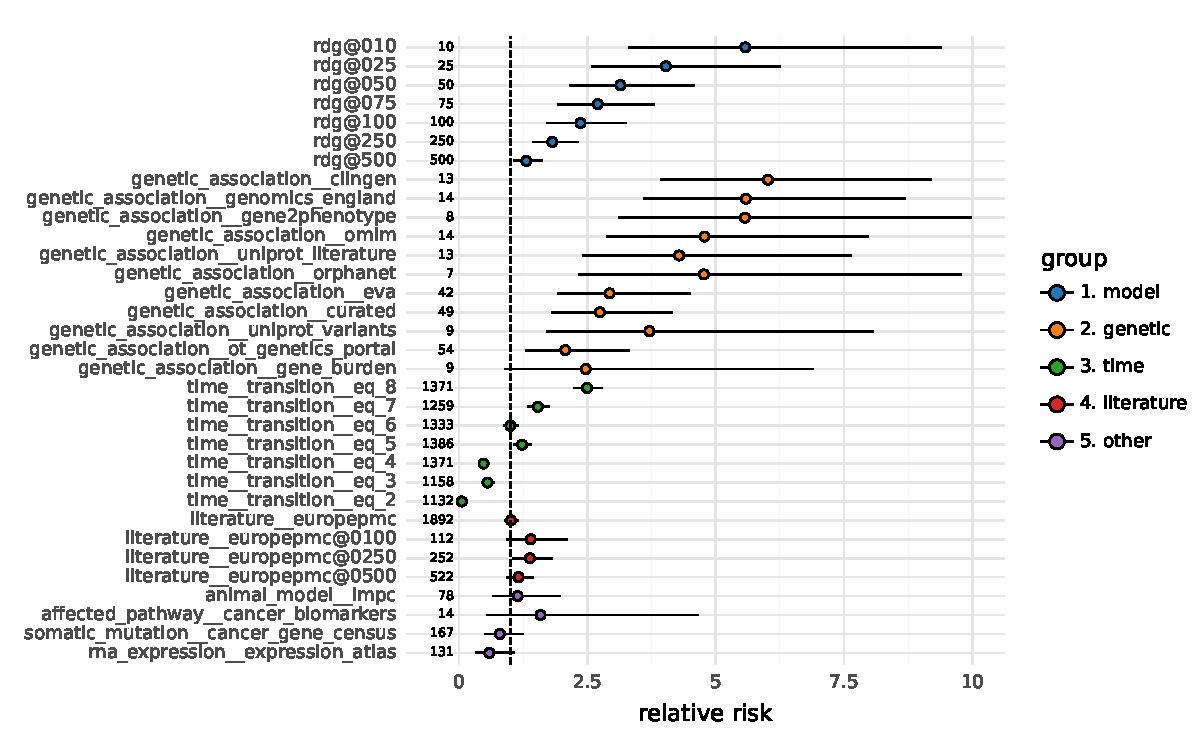
\includegraphics[width=1\textwidth]{relative_risk_core_features.pdf}
  \caption{
    \textbf{Performance of individual features and predictive scores as measured by relative risk}.
    RDG model results denoted by \colorbox{Gainsboro}{rdg@N} correspond to results for the \colorbox{Gainsboro}{N} top TD pairs. The same convention is used for \colorbox{Gainsboro}{literature} evidence and the \colorbox{Gainsboro}{time\_\_transition\_\_eq\_X} convention denotes RR estimates when the time since the phase 2 transition is equal to \colorbox{Gainsboro}{X} years. All other features are assessed based on their existence. The counts along the origin indicate how many TD pairs were used to compute the RR numerator.
  }
  \label{fig:relative_risk_core_features}
\end{figure}


\begin{figure}
  \centering
  \captionsetup{width=.9\linewidth}
  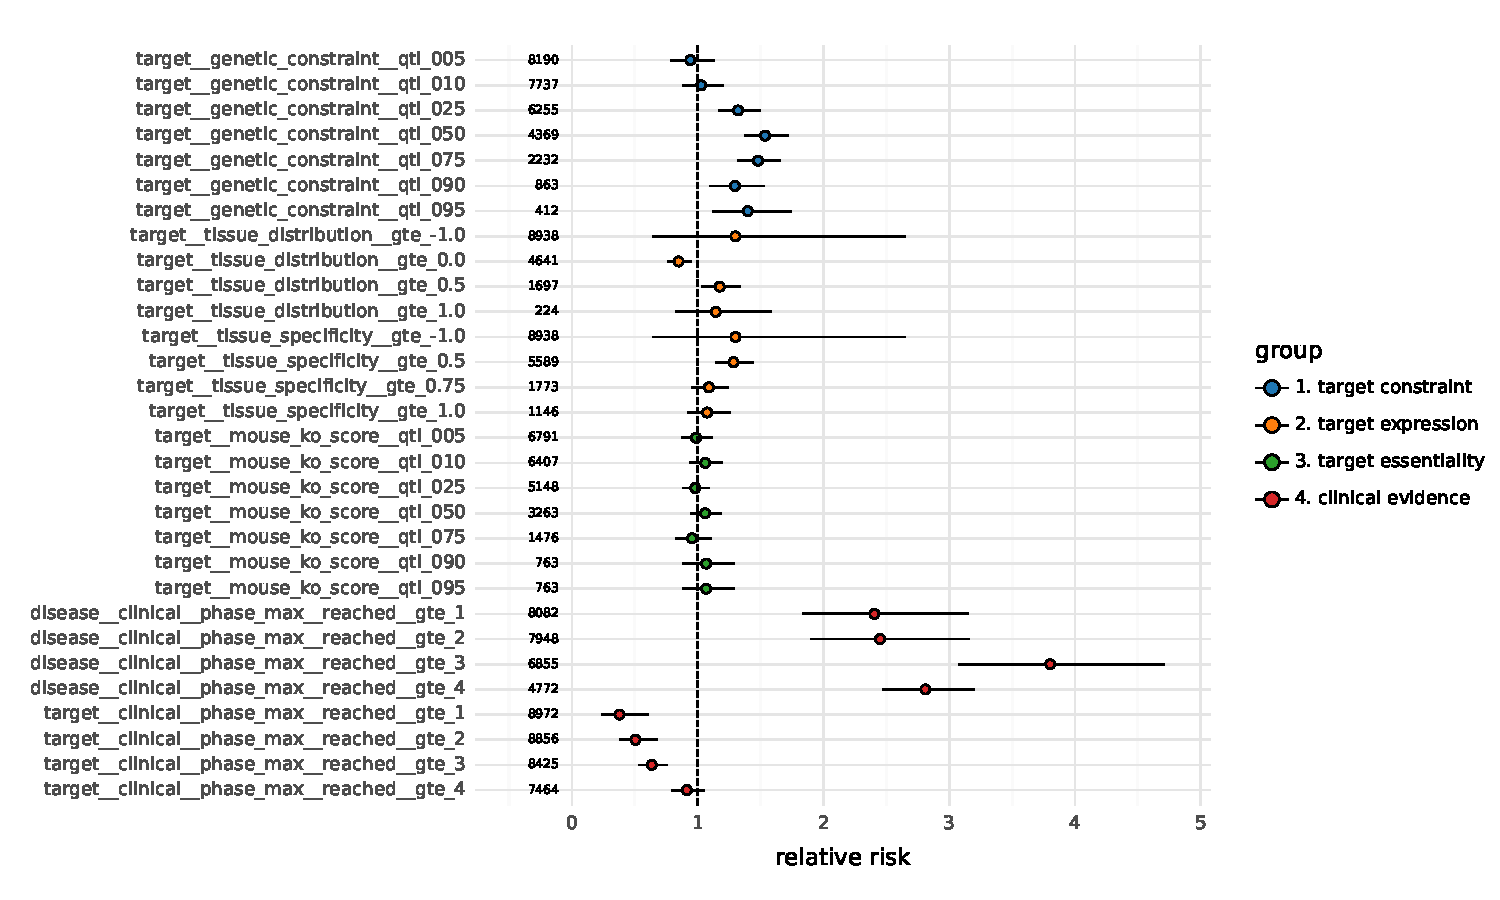
\includegraphics[width=1\textwidth]{relative_risk_static_features.pdf}
  \caption{
    \textbf{Relative risk scores for target/disease features}.
    The features ending with \colorbox{Gainsboro}{qtl\_Q} denote binary indicators constructed from cases where the feature meets or exceeds quantile \colorbox{Gainsboro}{Q} of its distribution. The features ending with \colorbox{Gainsboro}{gte\_X} denote indicators for when the feature meets or exceeds a specific value \colorbox{Gainsboro}{X}.
  }
  \label{fig:relative_risk_static_features}
\end{figure}


\begin{figure}
  \centering
  \captionsetup{width=.9\linewidth}
  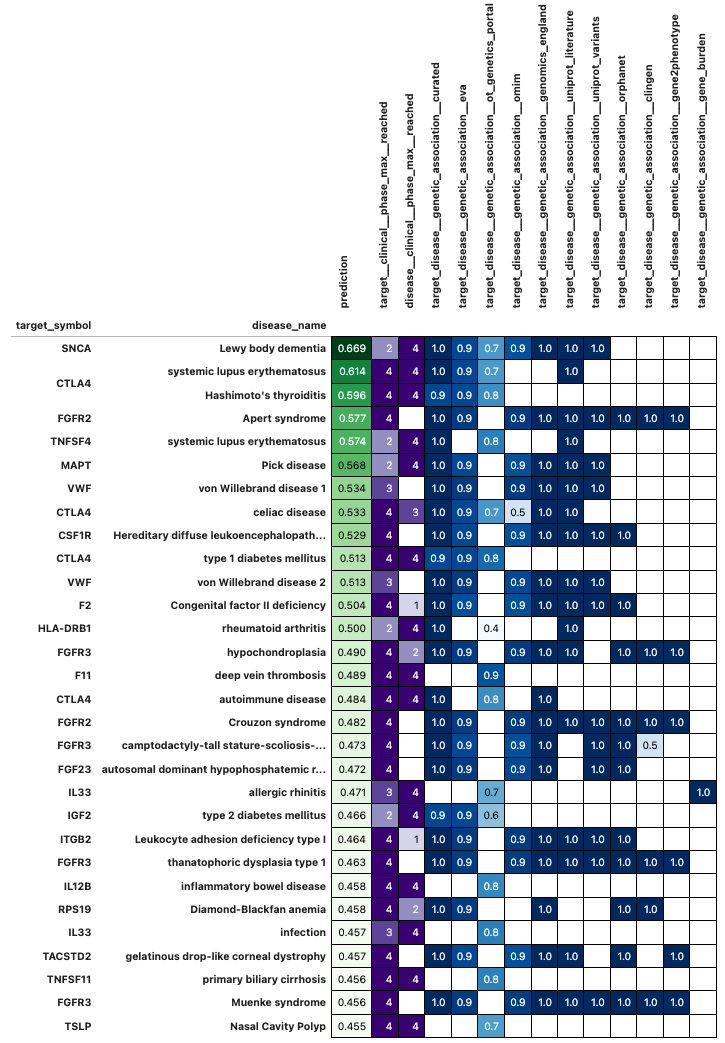
\includegraphics[width=.9\textwidth]{top_opportunity_predictions.png}
  \caption{
    \textbf{Top ranked undeveloped, tractable target-disease pairs}. The highest scoring TD pairs per the RDG model that have not entered clinical trials despite having a target that has been in trials of an antibody-based drug. All values shown other than \textbf{prediction} are raw feature values, unweighted by RDG coefficients.
  }
  \label{fig:top_opportunity_predictions}
\end{figure}


\begin{figure}
  \centering
  \captionsetup{width=.9\linewidth}
  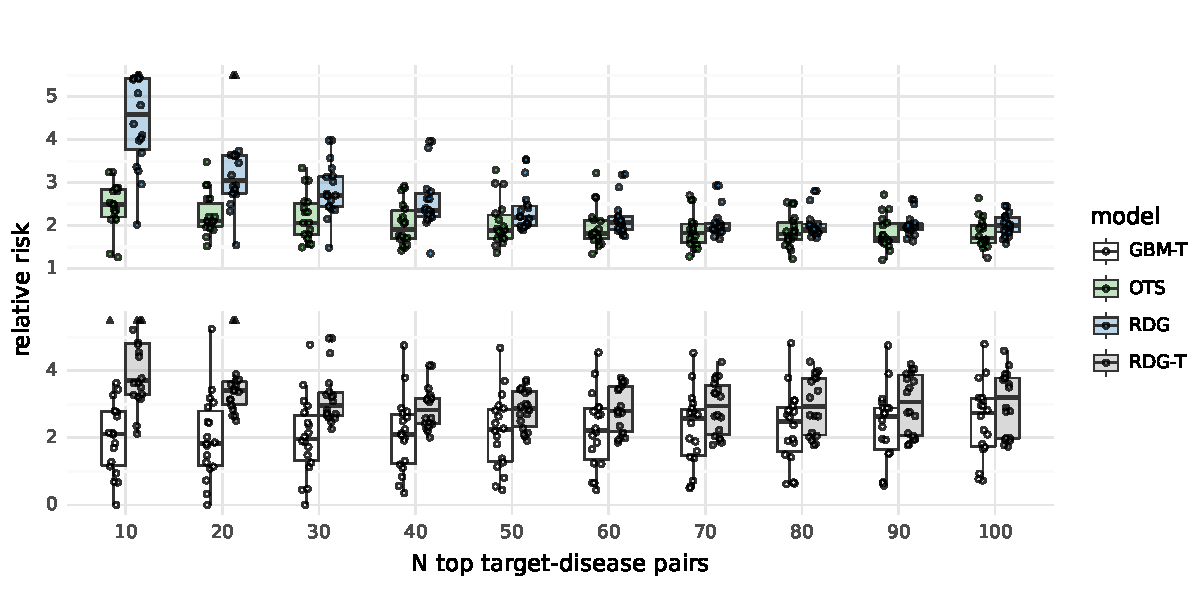
\includegraphics[width=1\textwidth]{sensitivity_relative_risk.pdf}
  \caption{
    \textbf{Relative risk distributions across configurations in sensitivity analysis}.
    The distribution of the mean RR values displayed for a single configuration in Figure~\ref{fig:performance_across_ta} is shown here across 18 configurations.
  }
  \label{fig:sensitivity_relative_risk}
\end{figure}

\begin{figure}
  \centering
  \captionsetup{width=.9\linewidth}
  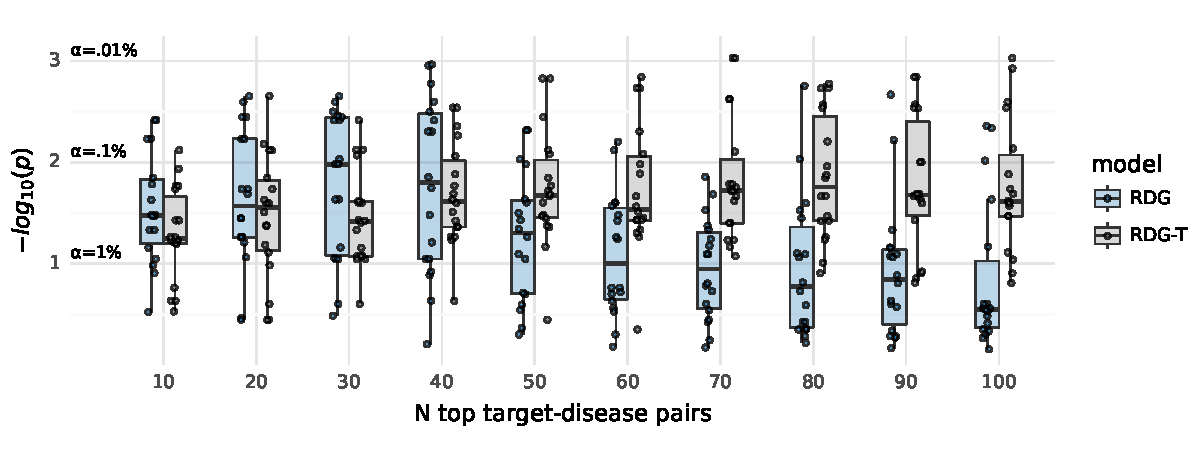
\includegraphics[width=1\textwidth]{sensitivity_p_values.pdf}
  \caption{
    \textbf{P-value distributions across configurations in sensitivity analysis}.
    The distribution of the p-values displayed for a single configuration in Supplementary~Figure~\ref{fig:relative_risk_dist_across_ta} is shown here across 18 configurations.
  }
  \label{fig:sensitivity_p_values}
\end{figure}


\bibliographystyle{unsrt}  
\bibliography{references} 

\end{document}
